Following from Section \ref{design}, this section aims to ... // TODO - complete the intro paragraph to the implementation section.

\subsection{Interfacing With Raspberry Pi SBC}

Due to security reasons, also noted by Shepherd, it is not possible to connect the RPi SBC to the Eduroam University network. This incurs a major roadblock, preventing remote communication to the RPi via SSH and communications to the internet from the RPi. Two aspects will ensure complete and seamless connectivity of the system: (a) SSH connection from the laptop to the RPi to enable remote connectivity for configuration and control, and (b) internet connection from the RPi to a valid network to enable the installation and update of the OS and other software. The security policies in place across all University-owned networks block communication between devices. Therefore, there must be a separate link between the RPi and the device to initiate an SSH connection. As Figure \ref{fig:pi_interfacing} illustrates, SSH communications will occur over an Ethernet connection between the RPi and a personal computer, and internet communications will occur over Wi-Fi to a separate University of York-owned network called `mydevices', which is intended for internet access from games consoles and specific smart home devices, and can be connected to by registering the RPi SBC's MAC address via a web portal and then entering a default Wi-Fi WPA2 Personal password on the RPi.

\begin{figure}[H]
    \centering
    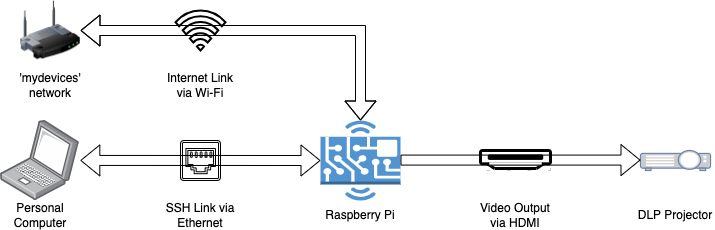
\includegraphics[width=1\textwidth]{assets/interface_diagram.png}
    \caption{Illustration of the Raspberry Pi SSH and Wi-Fi communication configuration, including video output interfacing with HDMI.}
    \label{fig:pi_interfacing}
\end{figure}

The RPi must have a set hostname for easy identification, and through NetworkManager, configuring `wlan0' to connect to the `mydevices' access point for internet access, and to prevent random and intermittent SSH disconnections and unresponsiveness, configuring `eth0' to a static IP address in the format 192.168.0.xxx/24 and disabling IPv6. Creating a new network on the personal computer (PC) using the Ethernet interface with DCHP disabled, IP address set to 192.168.0.1/24, and subnet mask set to 255.255.255.0, ensures a bidirectional communication channel via Ethernet between the PC and RPi, essential for SSH. Unlike Shepherd's system, which uses the Raspberry Pi OS, this system utilises the Raspberry Pi OS Lite which lacks a desktop environment. Using SSH with X11 forwarding with an X11 display server software, such as XQuartz, on the PC, graphical user interface windows will render on the PC, enabling quick system debugging. Due to the lack of a desktop environment, video output to the DLP projector will be possible by directly writing to the Framebuffer, which is a portion of memory in RAM containing a bitmap that drives the video display output, ensuring display output rates quicker than through a GUI window such as in Shepherd's system.

\subsection{Backscatter Simulator for Synthetic Ground Truth}

This software, code in Appendix \ref{sim_code}, utilises Python 3.11.2 just like the rest of the Python programs in this project, the `Pygame' package, which is a game library, to render the graphical user interface, the `random' package to generate randomised particle velocities, the `uuid' package to generate a unique ID for each particle in the simulation, and the `csv' package to generate an export dataset consisting of the positions and radii of each particle at every simulated frame. Defining a set of constants at the start to control the simulation parameters, which Table \ref{table:simbubbleclassparams} describes, the script also consists of a `Bubble' class which denotes a backscatter particle, with the class fields in Table \ref{table:simbubbleclassfields} and the class methods in Table \ref{table:simbubbleclassfuncs}, all tables in Appendix \ref{sim_tbls}.

The program flow, illustrated in Figure \ref{fig:simflow}, begins by initialising the Pygame module and creating the graphical window and the simulation clock. If the program is not set to generate the bubble backscatter particles continuously, the program will initialise the bubble backscatter particles, ensuring that the bubble limit is reached before entering the simulation loop. Within the simulation loop, as each iteration denotes a new frame, the program initialises the simulation window background with the colour defined by the user in the constant. Next, only if the constant particle generation feature is enabled by the user, the program initialises the bubbles to the maximum count possible. Then, the program logs the position and radius of each backscatter particle in the frame before drawing every bubble and moving them. The program then runs a probability check, only if true will it randomise the velocities of every single bubble. The program then removes the particles that are outside of the simulation window before exporting an image capture of the frame. The reason behind exporting a PNG image file of each frame instead of a singular video file is to simulate the frame-by-frame capture logic of the Backscatter Cancellation System from the RPi GS Camera, Section \ref{system_impl} explains this in further detail. Finally, the Pygame-provided clock functionality limits the simulation to the user-defined constant and stores the time delta, which is the duration in seconds from the last frame, before iterating once again. When the user inputs a `quit' signal by closing the window, the program creates a CSV file, with the help of the `csv' Python module, by offloading the metric data from each frame before the program gracefully terminates.

\pagebreak
\begin{landscape}
    \begin{figure}
        \centering
        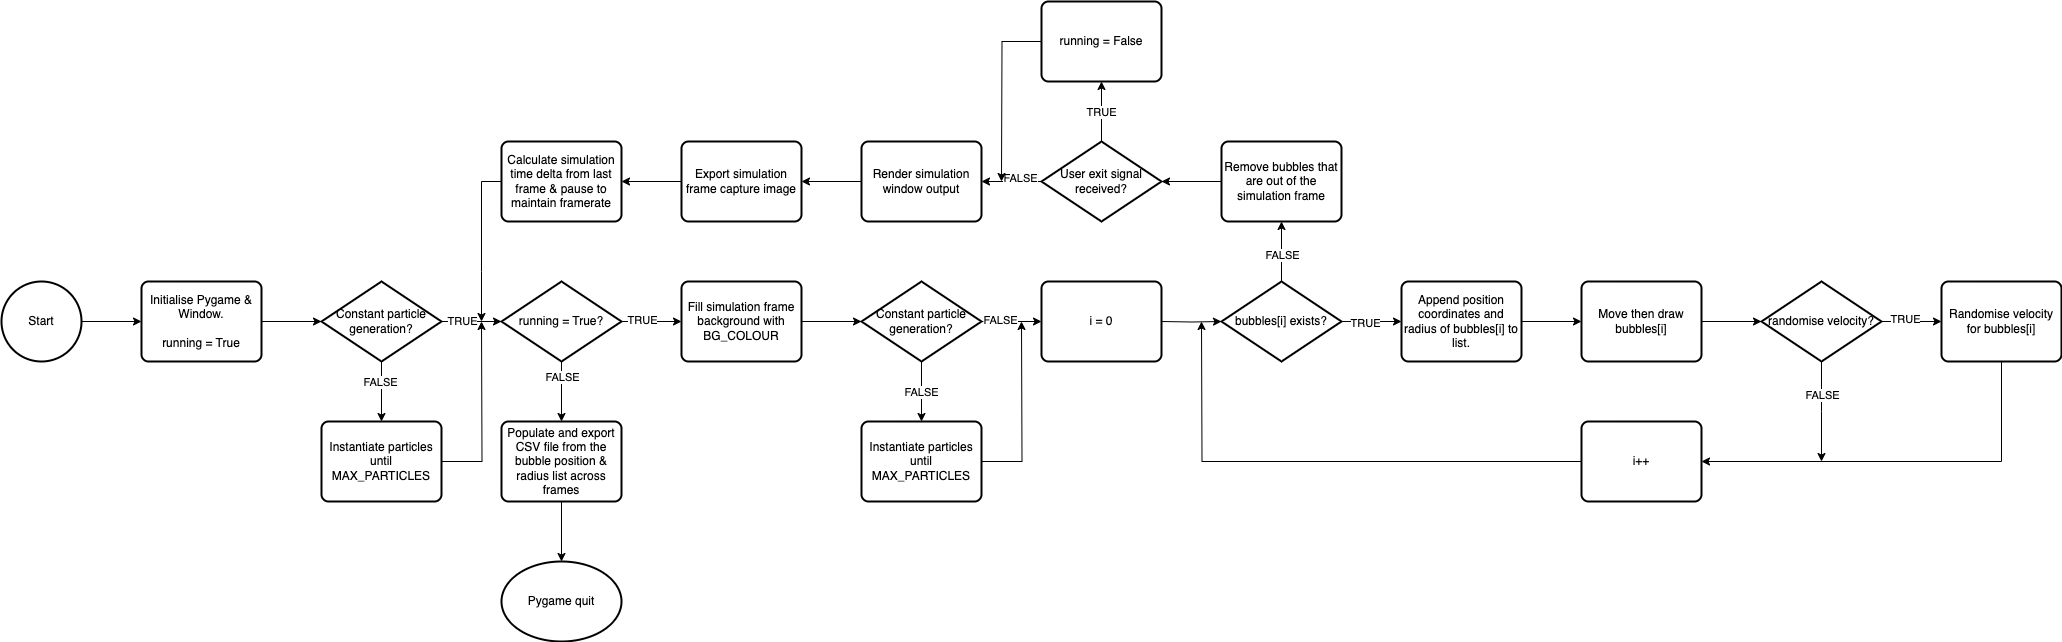
\includegraphics[width=1\linewidth]{assets/impl-sim_flow.png}
        \caption{Flowchart of backscatter simulation software process.}
        \label{fig:simflow}
    \end{figure}
\end{landscape}
\pagebreak

\subsection{Lossless Video Recorder for Physical Testing}
\label{pirec_impl}

As Section \ref{designrec} introduces, this software, Python scripts in Appendix \ref{rec_code}, records test footage of bubbles from the underwater testing facility at the Institute for Safe Autonomy using an RPi 5 and an RPi GS Camera, from the submersible system itself. The software also drives a DLP projector to project a fully illuminated white light source, ensuring a well-lit scene and to induce backscatter, via HDMI using the Framebuffer to eliminate the need for a desktop environment. Aside from the main entry point script, the software consists of three self-built modules: (1) ProjectorManager, which interfaces the software with the DLP projector via the Framebuffer, (2) the CameraManager, which interfaces the RPi Camera with the software, and finally, (3) the PreviewManager, which produces the GUI window to output the recording previews and program status. The program uses the `Numpy' Python package to generate bitmap arrays of pixel values to drive the DLP projector via the Framebuffer. The `Picamera2' library, although only available as a beta release at the time of writing, provides the program with high-level access to the RPi Cameras and RPi SBC's built-in imaging hardware. The `subprocess' package spawns the FFmpeg process to encode the recording, with the assumption that FFmpeg is present on the system's RPi SBC, and finally, the program uses the `OpenCV' package to access machine-vision algorithms for image processing and to generate the preview GUI window. The tables in Appendix \ref{rec_tbls} list and describe the program configuration constants, and the fields and methods for each class.

\begin{figure}[H]
    \centering
    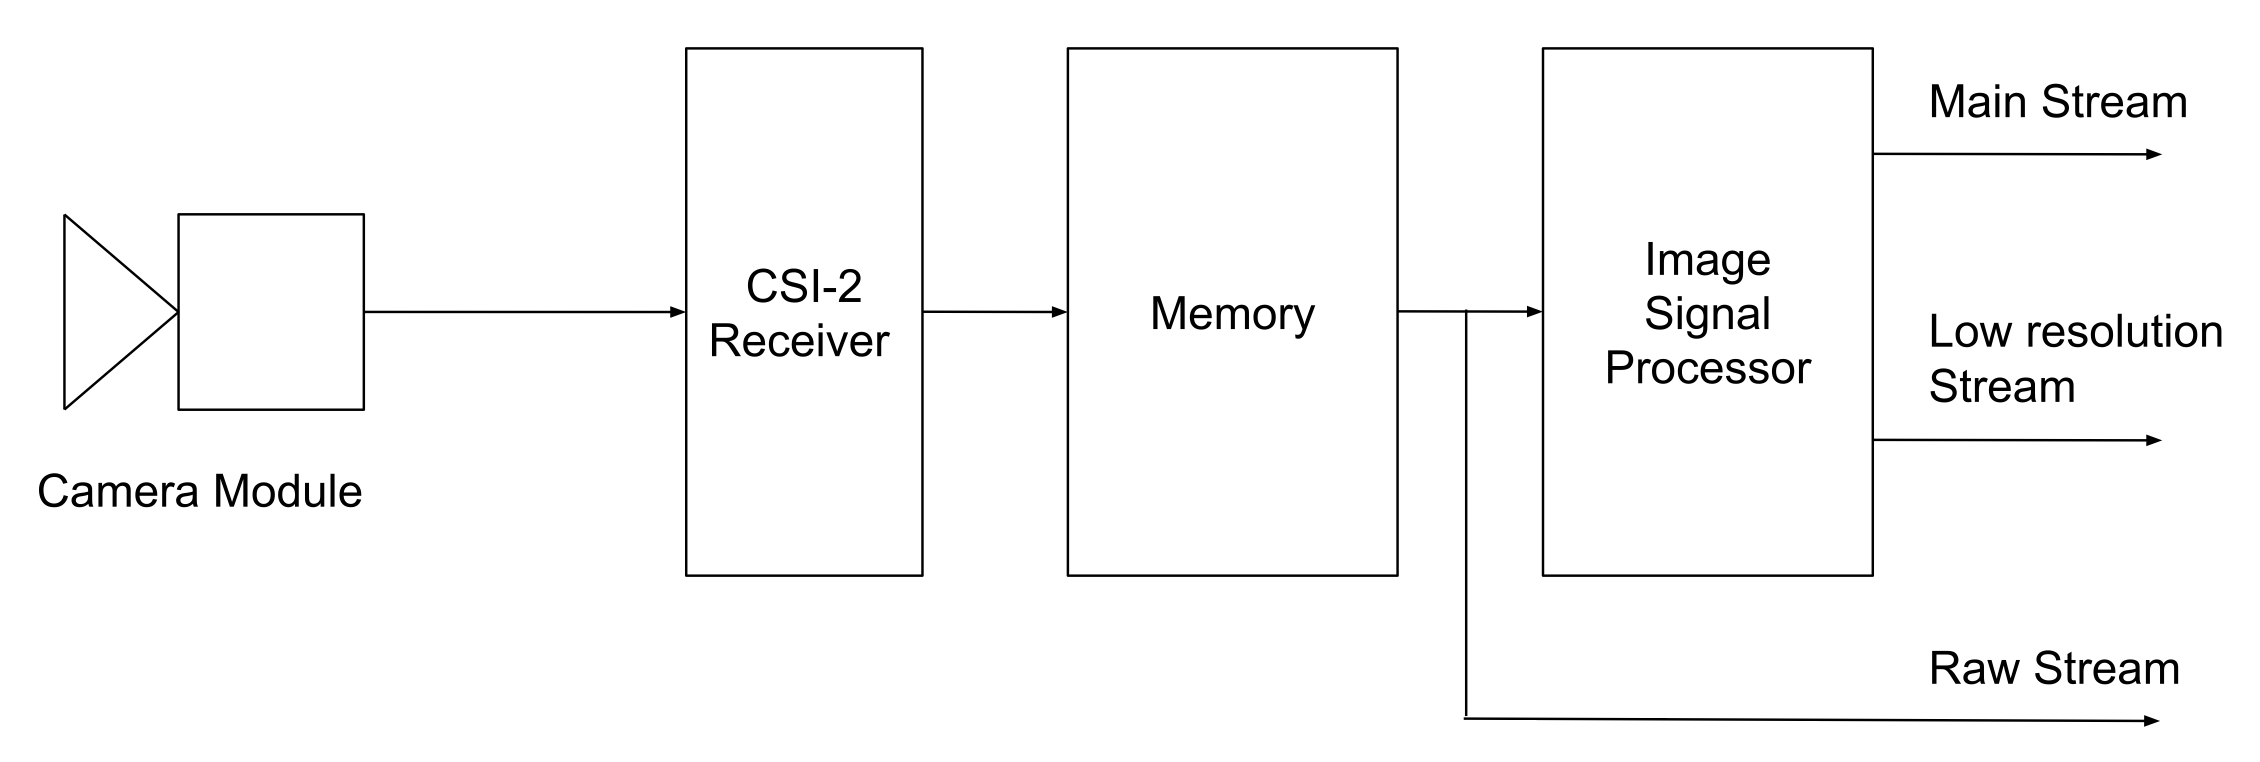
\includegraphics[width=1\textwidth]{assets/picamera-system.png}
    \caption{Illustration from \cite{raspberrypiltdPicamera2Library2024} of the Raspberry Pi camera system.}
    \label{fig:picam_system}
\end{figure}

As the Picamera2 library manual from \cite{raspberrypiltdPicamera2Library2024} illustrates, the RPi camera module delivers the output data stream, which is in native sensor format and not human-viewable, to the CSI-2 receiver hardware block onboard the RPi SBC via a ribbon cable. This hardware block transfers the incoming data into memory, ready for delivery to applications. In the initial prototyping stage for this system tool's implementation, I was receiving and recording the `raw' stream. However, this data required a lot of computationally intensive processing to convert to a human-viewable format, in addition to the high data throughput requirement of \SI{475}{\mega\byte} per second, recording at a steady rate was impossible even with a memory buffer. The Image Signal Processor (ISP) onboard the RPi SBC reads the `raw' stream from memory and efficiently cleans and processes the pixel data stream, ultimately producing a human-viewable output in either, depending on user set configuration, the RGB or YUV format. Instead of parsing the `raw' stream, I chose to process the `main' output stream in the final version of the software, configuring the exact resolution and framerates, in addition to a BGR888 output format such that the data is natively compatible with the OpenCV image processing libraries.

Figure \ref{fig:recflow} illustrates the flow of the software. The program begins with an initialisation, initialising the preview window, which passes through to the remote SSH connection on the PC via X11 forwarding, the projector via the Framebuffer, and the Picamera2 library, which applies a configuration to the RPi GS camera module and starts it. The main loop of the program then begins, retrieving the ISP-processed camera sensor array from the `main' output stream, and also retrieving the statuses of whether the projector light is on and whether the camera is recording. The sensor array frame is sent to the preview window, along with the statuses that the program overlays on the camera frame, finally logging any user-input keypresses. Using the Framebuffer, which is a memory location accessible through a directory, the program can toggle the light source by writing a bitmap array of white pixel values to turn on, and a bitmap array of black pixel values to turn off. If the program detects an `L' keypress, the projector light source toggles. With an `R' keypress, the program toggles the recording status. If the recording needs to start, the program initialises a memory buffer, configures the Picamera2 module to write to this Framebuffer along with a `Null' encoder, which ensures that the output is unencoded and `raw', and finally sends a signal to start recording. If the recording needs to stop, the program sends a signal to the Picamera2 module to stop the current recording, and using FFmpeg, which is installed on the RPi SBC, the program applies lossless encoding using the FFV1 encoder to convert the bitstream into an `.MKV' file, reducing the filesize and converting to a common video file format, for easy file transmission and so that any general-purpose software can open and this footage for playback. When the program receives an `E' key input, it will send the shutdown signal to the Picamera2 module, which gracefully terminates the camera module, it will turn off the projector light source by clearing the Framebuffer and sends a `destroy windows' signal to OpenCV which will consequently close all windows gracefully, and finally, the program exits the main loop and quits. If the program does not detect a keypress, or if it has finished handling the keypress for all inputs except the exit signal, the main loop iterates such that the entire process repeats.

\pagebreak
\begin{landscape}
    \begin{figure}
        \centering
        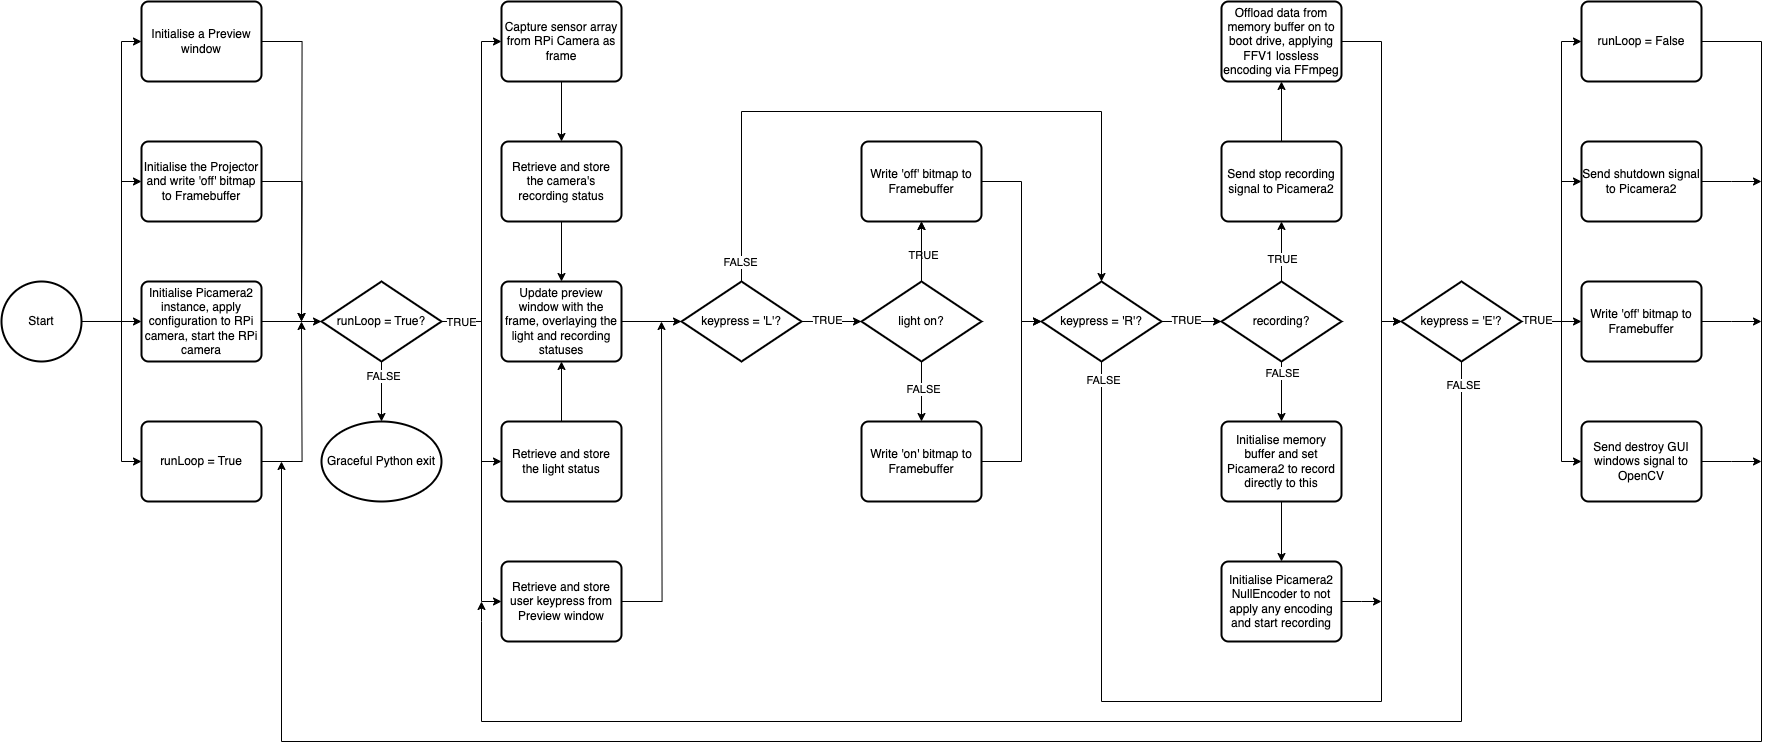
\includegraphics[width=1\linewidth]{assets/impl_rec-flow.png}
        \caption{Flowchart of lossless video recorder software process.}
        \label{fig:recflow}
    \end{figure}
\end{landscape}
\pagebreak

\subsection{Underwater Backscatter Cancellation System}
\label{system_impl}

The backscatter cancellation software, as Section \ref{designsystem} describes, with code and references for methods and fields in Appendix \ref{sys}, applies an image processing pipeline to segment backscatter particle regions to then generate light patterns for selective illumination using the DLP projector. Similar to the Lossless Video Recorder implementation in Section \ref{pirec_impl}, this system follows the object-oriented paradigm for modular code, breaking down the implementation into four self-built modules, aside from the entry point: (1) CaptureManager, which contains multiple different classes for input types, for example, a Raspberry Pi Camera interface similar to the CameraManager in Lossless Recorder, and a video file stream, which allows test footage inputs. (2) BSManager, which contains the image processing pipeline and backscatter segmentation functionalities, (3) TimeManager, which contains functionality to precisely time code, and finally, (4) WindowManager, very similar to PreviewManager in the Lossless Recorder program, contains functionality to output frames to a GUI for debugging. Instead of utilising the Picamera2's recording functionality for the RPi Camera Stream class, the system captures each frame individually at each iteration so enable fine control over framerates.  Due to time constraints and issues with system offsets/parallax, which Section \ref{testing} will explain in further detail, I couldn't implement functionality to output the light patterns by directly driving the DLP projector with parallax and offset mitigation, and therefore, skipping the implementation of logic to limit the framerates, such that this system outputs entirely via the GUI windows. Just like the Lossless Recorder program, this system uses the OpenCV package for both the image processing functions and for GUI windows. The program also uses Numpy package for bitmap operations concerning the image frames, the Pandas package for large data set operations concerning the metrics that the system tracks, the `psutil' package to set the program `nice' value, which is the software priority for the OS scheduler, and finally, the `time' package, where the system harnesses the performance counter, which is a system clock with the highest available resolution, to measure code execution durations.

As Figure \ref{fig:sysflow} illustrates, the program begins by setting the software priority level, this priority level is also called the `niceness', which has the lowest compatible value of -20, denoting the highest priority, and the highest compatible value of 0, denoting lowest priority, such that the lower priority processes demands less CPU processing time and are nicer to other processes in the system. Next, the program sets the correct input stream type before initialising the graphical preview windows and entering the main system loop. Within this loop, the program captures a frame from the input stream at the start of each iteration, and for each frame, applies the image processing pipeline to segment bubbles. After a greyscale conversion, Gaussian blur, and histogram equalisation, all using OpenCV functions, the program configures the Canny edge detection algorithm following the zero-parameter approach by \cite{rosebrockZeroparameterAutomaticCanny2015}. This approach by Rosebrock, simplifies the upper and lower Canny algorithm thresholds into a single parameter, sigma, which denotes a multiplier for the median pixel intensity of the input frame, such that the upper threshold is sigma above the median, and the lower threshold is sigma below the median. While not exactly zero-parameter as Rosebrock states, as there is still a sigma parameter, this approach ensures that the edge detection adapts to the specific characteristics of the input image even in different conditions, providing effective edge maps without manual parameter tuning. The system passes the Canny output, a bitmap of detected edges, to the segmentation method which then begins by finding contours, which are curves that join all the continuous points along a boundary, using OpenCV's \texttt{findContours()} method. Next, the program sends each contour detection to OpenCV's \texttt{minEnclosingCircles()} method, calculates the smallest enclosing circle for a set of contour points, and returns the center and radii of each circle. These minimum enclosing circles (MECs) will be the black `holes' in the white light patterns, ensuring the backscatter particles are dark whilst the system fully illuminates the surrounding environment. The program renders all of the output image frames, including those from the intermediate image processing pipeline stages if the debug window option is `True', whilst logging the user-input keypresses. If the user enters the `E' key, the program breaks from the main loop and enters the shutdown sequence. The program tracks the execution duration of each image processing stage with the performance counter for each frame, including metrics on the number of MEC detections, and the total frame processing time. When the program reaches the shutdown sequence, it extracts all of the metrics and generates a CSV export file, then exits all GUI windows, sends a shutdown signal to the RPi camera module, and finally exits completely.

\pagebreak
\begin{landscape}
    \begin{figure}
        \centering
        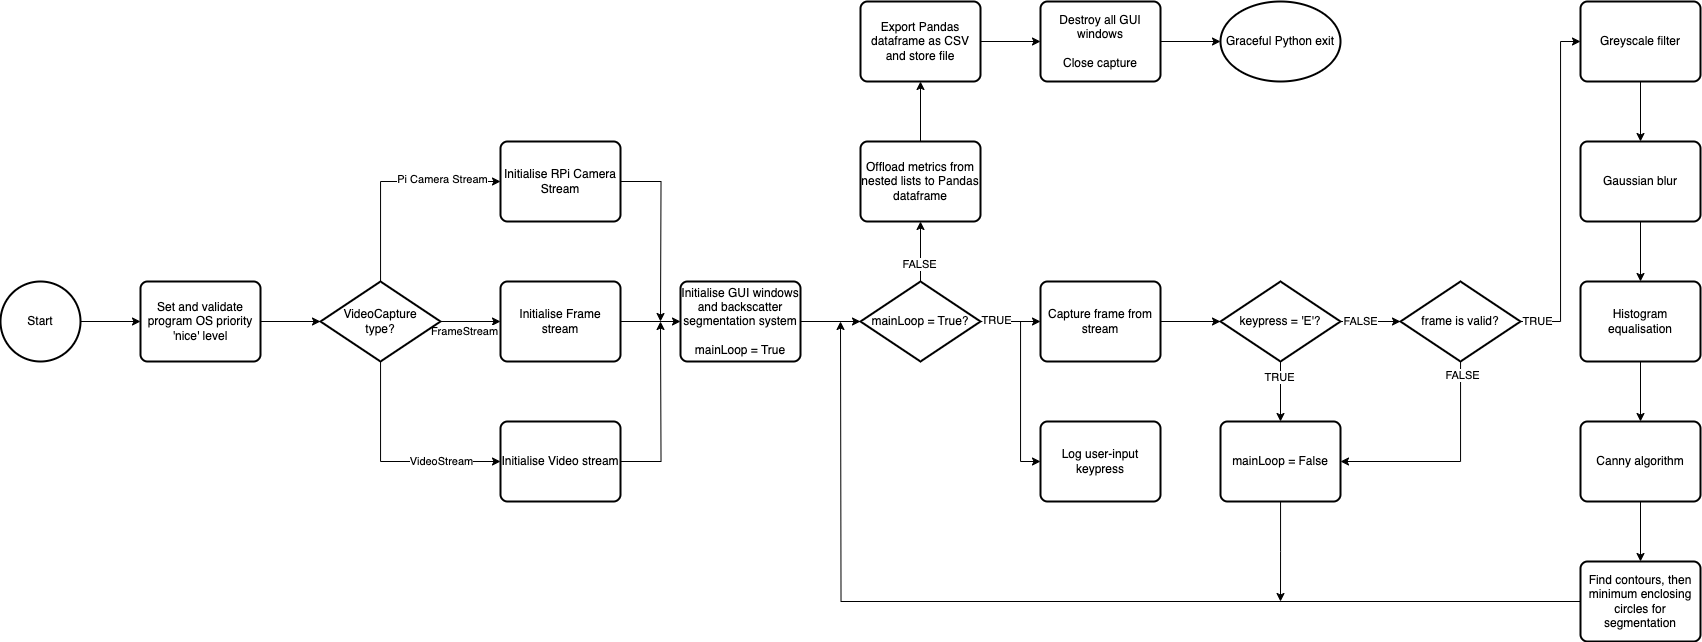
\includegraphics[width=1\linewidth]{assets/impl_system-flow.png}
        \caption{Flowchart of backscatter cancellation system software process.}
        \label{fig:sysflow}
    \end{figure}
\end{landscape}
\pagebreak

\subsubsection{Implementing Multiprocessing}

The functionality of the multiprocessing system follows very closely to the aforementioned base system, which only utilises a single thread due to the Python GIL limitations. Appendix \ref{mpsys} contains the references for methods and fields as well as the code for this implementation. The `multiprocessing' Python package provides an interface to support spawning subprocesses with concurrency, effectively side-stepping the GIL, and ultimately enabling the system to fully leverage multiple processors on a given machine, unlike Shepherd's system which employs `multithreading' and, therefore, is subject to the GIL for standard CPython execution. The single-thread version of the system is split into eight stages, denoted by classes that inherit the `multiprocessing' Process, which is an object that spawns as a separate process: (1) Capture, which first initialises the input stream, then enters an infinite loop that iterates until the input stream ends whilst returning the capture frame and any user-input keypresses. (2) Greyscale, which simply applies the greyscale filter. (3) Histogram Equalisation, which also simply applies histogram equalisation. (4) Gaussian Blur, again simply applying a Gaussian blur. (5) Canny Algorithm, which applies the Canny edge detector using the `zero-parameter' approach by Rosebrock. (6) Segmentation, which first finds the contours before applying the minimum enclosing circle function to segment the bubbles. (7) Project, which originally intended to output the light patterns to the Framebuffer, however due to the aforementioned constraints and limitations, instead outputs to a graphical preview window. Finally, (8) Logging, which exports the metrics into a Pandas DataFrame, then into a CSV document.

Due to the asynchronicity of the processes, the system employs queues to send data between stages in a thread-safe manner, preventing instances of data corruption with shared memory locations such as standard variables due to clobbering, where a process overwrites data while another was reading the data. The Capture stage will start filling its output queue with frames, and if no frames are left, or if the process receives a `quit' signal from the user, it enqueues with a special code instead of a frame. This queue is input to the next stage, which is Greyscale, and this stage begins to dequeue, applying the greyscale filter, then enqueues to its output queue, and if it receives a quit code instead of a frame, it will shutdown itself after forwarding the code. This logic repeats across all the other stages.

\subsection{Applying the PREEMPT-RT Patch}

The latest version of Raspberry Pi OS Lite at the time I built the real-time kernel, which was on the 15\textsuperscript{th} of March 2024, used the 6.6.20 Linux kernel version. Therefore, I applied the PREEMPT-RT patch with the corresponding version label of 6.6.20-rt25. I selected the `Fully Preemptible Kernel (Real-Time)' option, also enabling the RCU priority boosting with a 500ms delay boosting for the RT kernel and enabled the `Multi-core scheduler support' option for both RT and the non-RT kernel. Finally, I built both kernels, copied the libraries and both kernel image files into the correct RPi SBC directories, making sure to take a backup of the existing kernel, and finally, in the boot configuration file, I selected the correct kernel filename, being able to interchange between either of the two kernels, after rebooting.
